\section{Řešení projektu}

Implementace jednotlivých úkolů a dílčích částí řešení probíhala postupně. Nejdříve bude představen globální pohled na architekturu programu, následně chronologicky vytvořené části.

% program celkově
Program řídící činnost robota byl implementován v~jazyce C++ a ve své architektuře s~drží zvyklosti systému ROS2 \cite{ros} používat uzly (\textit{ROS nodes}), které mají různé zodpovědnosti. V~našem řešení existuje jeden hlavní uzel (\texttt{main node}), který sbírá informace ze svých vstupních uzlů a publikuje pokyny pro uzly, které sledují jeho výstupy. 

\begin{figure}[h]
    \centering
    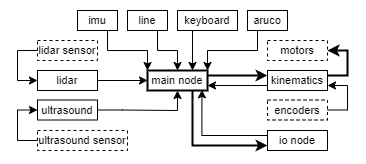
\includegraphics[width=0.45\textwidth]{images/nodes_schematic.png}
    \caption{Program z~celkového pohledu}
    \label{fig:program_obr}
\end{figure}

Celkový pohled na komunikaci námi vytvořených uzlů je ukázán na Obrázku \ref{fig:program_obr}. Uzly přímo napojené na hlavní uzel jsou nakresleny plnou čarou a komunikace přímo ovlivňující vnější stav robota je vyznačena tlustšími šipkami. Je vhodné zde také zmínit, že většina uzlů na obrázku dále interaguje se systémovými uzly robota, které již byly pro naši implementaci předpřipraveny.

% kinematika
Aby byl robot schopen řízeného pohybu, byl implementován uzel \texttt{kinematics}, který se stará o~kinematiku diferenciálního podvozku a využívá pomocné uzly \texttt{motors} a \texttt{encoders}. Uvnitř tohoto uzlu jsou mj. zadány vlastnosti robota vypsané v~Tabulce \ref{tab:vlastnosi}.

\begin{table}[]
    \centering
    \begin{tabular}{|l|l|}
        \hline
        \textbf{Vlastnost} & \textbf{Hodnota} \\ \hline
        Poloměr kola & 33 mm \\ \hline
        Obvod kola & 20,73 mm \\ \hline
        Rozchod kol & 128 mm \\ \hline
        Pulzy enkodéru & 576 za rotaci \\ \hline
    \end{tabular}
    \caption{Vlastnosti robota}
    \label{tab:vlastnosi}
\end{table}

% čára a PID
Jízda po čáře je pak implementována v~uzlu \texttt{line}, a to s~řízením typu \textit{bang-bang} i s~řízením pomocí PID regulátoru (jehož implementaci využíváme i v~dalších uzlech). Konkrétní hodnoty jednotlivých složek regulátoru jsou ${K_p=1}$; ${K_i=0,001}$ a ${K_d=0,1}$. Za zmínku také stojí, že po spuštění naší implementace sledování čáry provede robot na počátku kalibrační pohyb, při kterém určí aktuální hodnoty dosažitelné na čáře a mimo ni. Tím je schopen se přizpůsobit různým světelným podmínkám i různým odstínům povrchu a čáry.

% ultrazvuk
Obdobně je implementován i pohyb koridorem s~pomocí ultrazvukových senzorů, tedy existuje i \textit{bang-bang} verze i PID verze řízení průjezdu. Složky PID (resp. PD) regulátoru zde mají hodnoty ${K_p=1}$; ${K_i=0}$ a ${K_d=0,4}$. Ultrazvukové senzory jsou znovu využity i u~implementace jízdy v~koridoru s~pomocí LiDARU, kde se aktivují v~případě přílišného přiblížení ke stěně chodby (v~naší implementaci vždy, když LiDAR přestává fungovat spolehlivě a vrací neplatné výsledky).

\begin{figure}[h]
    \centering
    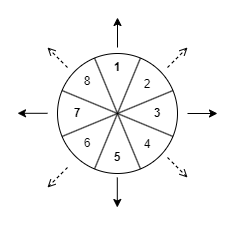
\includegraphics[width=0.25\textwidth]{images/lidar_circle.png}
    \caption{Rozdělení laloků LiDARu}
    \label{fig:lidar_obr}
\end{figure}

% lidar
U~průjezdu chodbou s~pomocí LiDARu jsme opět implementovali i \textit{bang-bang} i PID řízení, pro pozdější pohyb bludištěm ale využíváme pouze PID regulátor (lépe řečeno PD, hodnoty složek jsou totožné s~těmi u~ultrazvukových senzorů). Jelikož LiDARová jednotka robota rotuje a snímá celé jeho okolí, pomyslný kruh je v~naší implementaci rozdělen na 8 výsečí, jak je znázorněno na Obrázku \ref{fig:lidar_obr}. Při běžném pohybu chodbou, kde je jeho cílem držet se v~jejím středu, využívá robot laloků označených sudými čísly a čárkovanými šipkami. Ve chvíli, kdy v~chodbě detekuje nepravidelnost (potenciální křižovatku), využije laloky označené lichými čísly a plnými šipkami pro určení jejího typu a následně své další trasy.

% vizualizace
Detekovanou vzdálenost, resp. přítomnost nepravidelnosti, robot v~naší implementaci signalizuje pomocí změny barvy světla zabudovaných LED. Změnou barvy světla jedné ze 4 diod také signalizuje vybraný směr další cesty.

% aruco
V~uzlu \texttt{aruco} se nachází implementace poslední dílčí části projektu, a to detekce a získání hodnoty ArUco kódů pomocí robotovy kamery. Největší část implementace obstarává knihovna OpenCV \cite{opencv}, kterou pro detekci a přečtení kódu naše implementace využívá. Uzel přečtenou hodnotu ArUco kódu pouze předává dál, aby ji měla k~dispozici část programu zabývající se řízením trasy robota.

% řešení bludiště
Konečným úkolem robota je projet bludištěm, což je v~naší implementaci řešeno dvěma strategiemi. První z~nich pouze určuje, že robot bude sledovat pravou stěnu bludiště (což časem vede k~nalezení cíle, jelikož se v~bludišti nenachází žádné smyčky) a druhá potom využívá přítomnosti ArUco kódů, které napovídají nejkratší cestu k~cíli. V~případě, že druhá strategie selže, např. z~důvodu „přehlédnutí“ kódu, aplikuje se druhá strategie – robot by měl tedy v~každém případě dorazit do cíle.

% ovládání klávesnicí
V~průběhu řešení projektu byla také navíc implementována možnost ovládat činnosti a jízdu robota s~pomocí klávesnice počítače (na čemž spolupracují uzly \texttt{keyboard} a \texttt{main node}). Různým činnostem byla přiřazena písmena, např. \texttt{L} spouští jízdu s~pomocí LiDARu a \texttt{U} s~pomocí ultrazvukových senzorů. Navíc je možné v~případě potřeby ovládat klávesami \texttt{W}, \texttt{A}, \texttt{S} a \texttt{D} pjízdu s~pomocí ultrazvuku ohyby vpřed, vlevo, vpravo a vzad.
